\documentclass{standalone}
\usepackage{tikz}
\usetikzlibrary{patterns, positioning}


\begin{document}
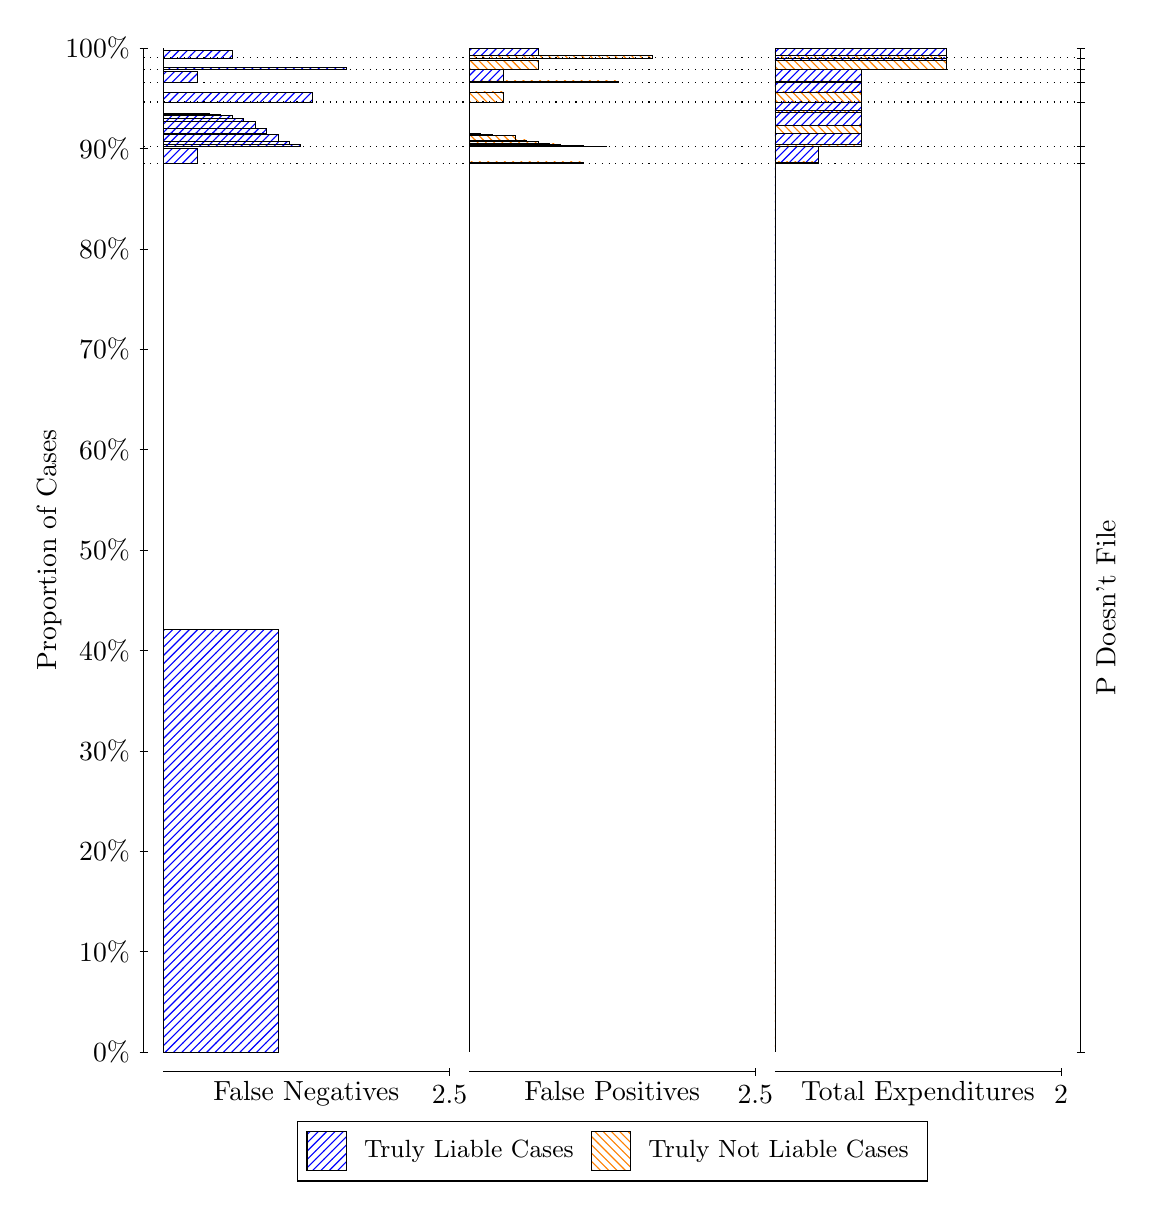
\begin{tikzpicture}
\draw[black, very thin] (1.5,1.75) -- (1.5,14.5);
\node[rotate=90, text=black, anchor=center] at (0.3, 8.125) {Proportion of Cases};
\draw[black, very thin] (1.45,1.75) -- (1.55,1.75);
\node[text=black, anchor=east] at (1.45, 1.75) {0\%};
\draw[black, very thin] (1.45,3.025) -- (1.55,3.025);
\node[text=black, anchor=east] at (1.45, 3.025) {10\%};
\draw[black, very thin] (1.45,4.3) -- (1.55,4.3);
\node[text=black, anchor=east] at (1.45, 4.3) {20\%};
\draw[black, very thin] (1.45,5.575) -- (1.55,5.575);
\node[text=black, anchor=east] at (1.45, 5.575) {30\%};
\draw[black, very thin] (1.45,6.85) -- (1.55,6.85);
\node[text=black, anchor=east] at (1.45, 6.85) {40\%};
\draw[black, very thin] (1.45,8.125) -- (1.55,8.125);
\node[text=black, anchor=east] at (1.45, 8.125) {50\%};
\draw[black, very thin] (1.45,9.4) -- (1.55,9.4);
\node[text=black, anchor=east] at (1.45, 9.4) {60\%};
\draw[black, very thin] (1.45,10.675) -- (1.55,10.675);
\node[text=black, anchor=east] at (1.45, 10.675) {70\%};
\draw[black, very thin] (1.45,11.95) -- (1.55,11.95);
\node[text=black, anchor=east] at (1.45, 11.95) {80\%};
\draw[black, very thin] (1.45,13.225) -- (1.55,13.225);
\node[text=black, anchor=east] at (1.45, 13.225) {90\%};
\draw[black, very thin] (1.45,14.5) -- (1.55,14.5);
\node[text=black, anchor=east] at (1.45, 14.5) {100\%};

\draw[black, very thin] (13.4,1.75) -- (13.4,14.5);
\draw[black, very thin] (13.35,1.75) -- (13.45,1.75);
\node[anchor=west] at (13.35, 1.75) {};
\draw[black, very thin] (13.35,13.034) -- (13.45,13.034);
\node[anchor=west] at (13.35, 13.034) {};
\draw[black, very thin] (13.35,13.249) -- (13.45,13.249);
\node[anchor=west] at (13.35, 13.249) {};
\draw[black, very thin] (13.35,13.815) -- (13.45,13.815);
\node[anchor=west] at (13.35, 13.815) {};
\draw[black, very thin] (13.35,14.062) -- (13.45,14.062);
\node[anchor=west] at (13.35, 14.062) {};
\draw[black, very thin] (13.35,14.225) -- (13.45,14.225);
\node[anchor=west] at (13.35, 14.225) {};
\draw[black, very thin] (13.35,14.375) -- (13.45,14.375);
\node[anchor=west] at (13.35, 14.375) {};
\draw[black, very thin] (13.35,14.5) -- (13.45,14.5);
\node[anchor=west] at (13.35, 14.5) {};

\draw[black, very thin, pattern color=blue, pattern=north east lines] (1.75,1.75) rectangle (3.2033,7.1194);
\draw[black, very thin, pattern color=orange, pattern=north west lines] (1.75,7.1194) rectangle (1.75,13.034);
\draw[black, very thin, pattern color=blue, pattern=north east lines] (1.75,13.034) rectangle (2.186,13.229);
\draw[black, very thin, pattern color=orange, pattern=north west lines] (1.75,13.229) rectangle (1.75,13.249);
\draw[black, very thin, pattern color=blue, pattern=north east lines] (1.75,13.249) rectangle (3.494,13.28);
\draw[black, very thin, pattern color=blue, pattern=north east lines] (1.75,13.28) rectangle (3.3487,13.313);
\draw[black, very thin, pattern color=blue, pattern=north east lines] (1.75,13.313) rectangle (3.2033,13.399);
\draw[black, very thin, pattern color=blue, pattern=north east lines] (1.75,13.399) rectangle (3.058,13.422);
\draw[black, very thin, pattern color=blue, pattern=north east lines] (1.75,13.422) rectangle (3.058,13.477);
\draw[black, very thin, pattern color=blue, pattern=north east lines] (1.75,13.477) rectangle (2.9127,13.571);
\draw[black, very thin, pattern color=blue, pattern=north east lines] (1.75,13.571) rectangle (2.7673,13.61);
\draw[black, very thin, pattern color=blue, pattern=north east lines] (1.75,13.61) rectangle (2.622,13.646);
\draw[black, very thin, pattern color=blue, pattern=north east lines] (1.75,13.646) rectangle (2.4767,13.657);
\draw[black, very thin, pattern color=blue, pattern=north east lines] (1.75,13.657) rectangle (2.3313,13.673);
\draw[black, very thin, pattern color=orange, pattern=north west lines] (1.75,13.673) rectangle (1.75,13.815);
\draw[black, very thin, pattern color=blue, pattern=north east lines] (1.75,13.815) rectangle (3.6393,13.933);
\draw[black, very thin, pattern color=orange, pattern=north west lines] (1.75,13.933) rectangle (1.75,14.062);
\draw[black, very thin, pattern color=blue, pattern=north east lines] (1.75,14.062) rectangle (2.186,14.203);
\draw[black, very thin, pattern color=orange, pattern=north west lines] (1.75,14.203) rectangle (1.75,14.225);
\draw[black, very thin, pattern color=blue, pattern=north east lines] (1.75,14.225) rectangle (4.0753,14.256);
\draw[black, very thin, pattern color=orange, pattern=north west lines] (1.75,14.256) rectangle (1.75,14.375);
\draw[black, very thin, pattern color=blue, pattern=north east lines] (1.75,14.375) rectangle (2.622,14.473);
\draw[black, very thin, pattern color=orange, pattern=north west lines] (1.75,14.473) rectangle (1.75,14.5);
\draw[black, very thin, pattern color=orange, pattern=north west lines] (5.6333,1.75) rectangle (5.6333,7.665);
\draw[black, very thin, pattern color=blue, pattern=north east lines] (5.6333,7.665) rectangle (5.6333,13.034);
\draw[black, very thin, pattern color=orange, pattern=north west lines] (5.6333,13.034) rectangle (7.0867,13.055);
\draw[black, very thin, pattern color=blue, pattern=north east lines] (5.6333,13.055) rectangle (5.6333,13.249);
\draw[black, very thin, pattern color=orange, pattern=north west lines] (5.6333,13.249) rectangle (7.3773,13.252);
\draw[black, very thin, pattern color=orange, pattern=north west lines] (5.6333,13.252) rectangle (7.232,13.254);
\draw[black, very thin, pattern color=orange, pattern=north west lines] (5.6333,13.254) rectangle (7.0867,13.261);
\draw[black, very thin, pattern color=orange, pattern=north west lines] (5.6333,13.261) rectangle (6.9413,13.267);
\draw[black, very thin, pattern color=orange, pattern=north west lines] (5.6333,13.267) rectangle (6.796,13.282);
\draw[black, very thin, pattern color=orange, pattern=north west lines] (5.6333,13.282) rectangle (6.6507,13.293);
\draw[black, very thin, pattern color=orange, pattern=north west lines] (5.6333,13.293) rectangle (6.5053,13.317);
\draw[black, very thin, pattern color=orange, pattern=north west lines] (5.6333,13.317) rectangle (6.36,13.333);
\draw[black, very thin, pattern color=orange, pattern=north west lines] (5.6333,13.333) rectangle (6.2147,13.392);
\draw[black, very thin, pattern color=blue, pattern=north east lines] (5.6333,13.392) rectangle (5.924,13.407);
\draw[black, very thin, pattern color=blue, pattern=north east lines] (5.6333,13.407) rectangle (5.7787,13.419);
\draw[black, very thin, pattern color=blue, pattern=north east lines] (5.6333,13.419) rectangle (5.6333,13.815);
\draw[black, very thin, pattern color=orange, pattern=north west lines] (5.6333,13.815) rectangle (6.0693,13.944);
\draw[black, very thin, pattern color=blue, pattern=north east lines] (5.6333,13.944) rectangle (5.6333,14.062);
\draw[black, very thin, pattern color=orange, pattern=north west lines] (5.6333,14.062) rectangle (7.5227,14.084);
\draw[black, very thin, pattern color=blue, pattern=north east lines] (5.6333,14.084) rectangle (6.0693,14.225);
\draw[black, very thin, pattern color=orange, pattern=north west lines] (5.6333,14.225) rectangle (6.5053,14.345);
\draw[black, very thin, pattern color=blue, pattern=north east lines] (5.6333,14.345) rectangle (5.6333,14.375);
\draw[black, very thin, pattern color=orange, pattern=north west lines] (5.6333,14.375) rectangle (7.9587,14.402);
\draw[black, very thin, pattern color=blue, pattern=north east lines] (5.6333,14.402) rectangle (6.5053,14.5);
\draw[black, very thin, pattern color=orange, pattern=north west lines] (9.5167,1.75) rectangle (9.5167,7.665);
\draw[black, very thin, pattern color=blue, pattern=north east lines] (9.5167,7.665) rectangle (9.5167,13.034);
\draw[black, very thin, pattern color=orange, pattern=north west lines] (9.5167,13.034) rectangle (10.062,13.055);
\draw[black, very thin, pattern color=blue, pattern=north east lines] (9.5167,13.055) rectangle (10.062,13.249);
\draw[black, very thin, pattern color=orange, pattern=north west lines] (9.5167,13.249) rectangle (10.607,13.272);
\draw[black, very thin, pattern color=blue, pattern=north east lines] (9.5167,13.272) rectangle (10.607,13.413);
\draw[black, very thin, pattern color=orange, pattern=north west lines] (9.5167,13.413) rectangle (10.607,13.516);
\draw[black, very thin, pattern color=blue, pattern=north east lines] (9.5167,13.516) rectangle (10.607,13.689);
\draw[black, very thin, pattern color=orange, pattern=north west lines] (9.5167,13.689) rectangle (10.607,13.706);
\draw[black, very thin, pattern color=blue, pattern=north east lines] (9.5167,13.706) rectangle (10.607,13.815);
\draw[black, very thin, pattern color=orange, pattern=north west lines] (9.5167,13.815) rectangle (10.607,13.944);
\draw[black, very thin, pattern color=blue, pattern=north east lines] (9.5167,13.944) rectangle (10.607,14.062);
\draw[black, very thin, pattern color=orange, pattern=north west lines] (9.5167,14.062) rectangle (10.607,14.084);
\draw[black, very thin, pattern color=blue, pattern=north east lines] (9.5167,14.084) rectangle (10.607,14.225);
\draw[black, very thin, pattern color=orange, pattern=north west lines] (9.5167,14.225) rectangle (11.697,14.345);
\draw[black, very thin, pattern color=blue, pattern=north east lines] (9.5167,14.345) rectangle (11.697,14.375);
\draw[black, very thin, pattern color=orange, pattern=north west lines] (9.5167,14.375) rectangle (11.697,14.402);
\draw[black, very thin, pattern color=blue, pattern=north east lines] (9.5167,14.402) rectangle (11.697,14.5);
\draw[black, dotted] (1.5,13.034) -- (13.4,13.034);
\draw[black, dotted] (1.5,13.249) -- (13.4,13.249);
\draw[black, dotted] (1.5,13.815) -- (13.4,13.815);
\draw[black, dotted] (1.5,14.062) -- (13.4,14.062);
\draw[black, dotted] (1.5,14.225) -- (13.4,14.225);
\draw[black, dotted] (1.5,14.375) -- (13.4,14.375);
\draw[black, very thin] (1.75,1.5) -- (5.3833,1.5);
\node[text=black, anchor=north] at (3.5667, 1.5) {False Negatives};
\draw[black, very thin] (5.3833,1.45) -- (5.3833,1.55);
\node[text=black, anchor=north] at (5.3833, 1.45) {2.5};

\draw[black, very thin] (5.6333,1.5) -- (9.2667,1.5);
\node[text=black, anchor=north] at (7.45, 1.5) {False Positives};
\draw[black, very thin] (9.2667,1.45) -- (9.2667,1.55);
\node[text=black, anchor=north] at (9.2667, 1.45) {2.5};

\draw[black, very thin] (9.5167,1.5) -- (13.15,1.5);
\node[text=black, anchor=north] at (11.333, 1.5) {Total Expenditures};
\draw[black, very thin] (13.15,1.45) -- (13.15,1.55);
\node[text=black, anchor=north] at (13.15, 1.45) {2};

\node[text=black, centered, rotate=90] at (13.72, 7.3922) {P Doesn't File};







\draw (7.449999999999999,1.5) node[draw=none] (baseCoordinate) {};
\begin{scope}[align=center]
        \matrix[scale=0.5, draw=black, below=0.5cm of baseCoordinate, nodes={draw}, column sep=0.1cm]{
            \node[rectangle, draw, minimum width=0.5cm, minimum height=0.5cm, pattern color=blue, pattern=north east lines] {}; &
            \node[draw=none, font=\small, text=black] (B) {Truly Liable Cases}; &
            \node[rectangle, draw, minimum width=0.5cm, minimum height=0.5cm, pattern color=orange, pattern=north west lines] {}; &
            \node[draw=none, font=\small, text=black] (B) {Truly Not Liable Cases}; \\
            };
\end{scope}

\end{tikzpicture}
\end{document}